\newpage
\section{METHODOLOGY}

\subsection{System Block Diagram}

\begin{figure}[h!]
        \centering
        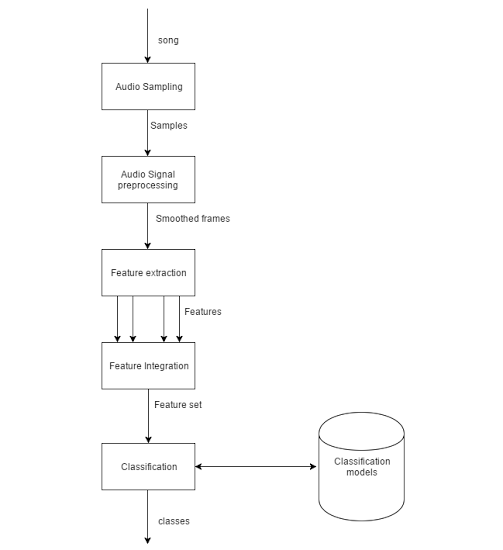
\includegraphics[width=130mm]{resources/mehang/methodology/systemblockdiagram}
        \caption{System block diagram}
\end{figure}

\subsection{Audio Sampling}
The central task that the Java sound API addresses is how to move bytes of formatted audio data into and out of the system. This task involves opening audio input and output devices and managing buffers that get filled with real-time sound data. It can also involve mixing multiple streams of audio into one stream (whether for input or output). The transport of sound into or out of the system has to be correctly handled when the user requests that the flow of sound be started, paused, resumed, or stopped.\\
\\
To support this focus on basic audio input and output, the Java Sound API provides methods for converting between various audio data formats, and for reading and writing common types of sound files. However, it does not attempt to be a comprehensive sound-file toolkit. A particular implementation of the Java Sound API need not support an extensive set of file types or data format conversions. Third-party service providers can supply modules that "plug in" to an existing implementation to support additional file types and conversions.\\
\\
The Java Sound API can handle audio transport in both a streaming, buffered fashion and an in-memory, unbuffered fashion. "Streaming" is used here in a general sense to refer to real-time handling of audio bytes.\\
\\
Major components of the java sound API are:
\begin{enumerate}[(i)]
        \item Formatted audio data refers to sound in any of a number of standard formats such as a data format which is represented by a Audioformat object which has the following attributes:
                \begin{itemize}
                        \item Encoding technique, usually pulse code modulation (PCM)
                        \item Number of channels (one for mono, two for stereo, etc.)
                        \item Sample rate (number of samples per second, per channel)
                        \item Number of bits per sample (per channel)
                        \item Frame rate
                        \item Frame size in bytes
                        \item Byte order (big-endian or little-endian)
                \end{itemize}
                The file format on the other hand is represented using the Audio File Format which has the following attributes
                \begin{itemize}
                        \item The file type (WAVE, AIFF, etc.)
                        \item The file's length in bytes
                        \item The length, in frames, of the audio data contained in the file
                        \item An AudioFormat object that specifies the data format of the audio data contained in the file
                \end{itemize}
                The Audio System class provides methods for reading and writing sounds in different file formats, and for converting between different data formats. Some of the methods let you access a file's contents through a kind of stream called an AudioInputStream .By reading a sound file as an AudioInputStream, you get immediate access to the samples, without having to worry about the sound file's structure (its header, chunks, etc.). A single method invocation gives you all the information you need about the data format and the file type.
        \item  Mixers which are used to handle one or more streams of audio input and one or more streams of audio output. In the typical case, it actually mixes together multiple incoming streams into one outgoing stream. A Mixer object can represent the sound-mixing capabilities of a physical device such as a sound card, which might need to mix the sound coming into the computer from various inputs, or the sound coming from application programs and going to outputs.
        \item A line which is an element of the digital audio which is a path for moving audio into or out of the system. Usually the line is a path into or out of a mixer Audio input and output ports are lines. These are analogous to the microphones and speakers connected to a physical mixing console. Another kind of line is a data path through which an application program can get input audio from, or send output audio to, a mixer. These data paths are analogous to the tracks of the multitrack recorder connected to the physical mixing console.One difference between lines in the Java Sound API and those of a physical mixer is that the audio data flowing through a line in the Java Sound API can be mono or multichannel (for example, stereo). By contrast, each of a physical mixer's inputs and outputs is typically a single channel of sound. To get two or more channels of output from the physical mixer, two or more physical outputs are normally used (at least in the case of analog sound; a digital output jack is often multichannel). In the Java Sound API, the number of channels in a line is specified by the AudioFormat of the data that is currently flowing through the line.
\end{enumerate}
Audio System serves as an application program's entry point for accessing these installed sampled-audio resources. You can query the Audio System to learn what sorts of resources have been installed, and then you can obtain access to them. For example, an application program might start out by asking the Audio System class whether there is a mixer that has a certain configuration, such as one of the input or output configurations illustrated earlier in the discussion of lines. From the mixer, the program would then obtain data lines, and so on.\\
\\
Here are some of the resources an application program can obtain from the Audio System:
\begin{itemize}
        \item \textbf{Mixers:} A system typically has multiple mixers installed. There is usually at least one for audio input and one for audio output. There might also be mixers that don't have I/O ports but instead accept audio from an application program and deliver the mixed audio back to the program. The Audio System class provides a list of all of the installed mixers.
        \item \textbf{Lines:} Even though every line is associated with a mixer, an application program can get a line directly from the Audio System, without dealing explicitly with mixers.
        \item \textbf{Format conversions:} An application program can use format conversions to translate audio data from one format to another.
        \item \textbf{Files and streams:} The Audio System class provides methods for translating between audio files and audio streams. It can also report the file format of a sound file and can write files in different formats.
\end{itemize}

\subsection{Audio Signal Pre-processing}
The preprocessing in music classification systems is used in order to increase the efficiency of subsequent feature extraction and classification stages and therefore to improve the overall system performance. Commonly the preprocessing includes the framing and window of the input signal. At the end of the preprocessing the smoothed frame are forwarded to the feature extraction stage.\\ 
\\
The general preprocessing pipeline is depicted in the following figure.
\begin{figure}[h!]
        \centering
        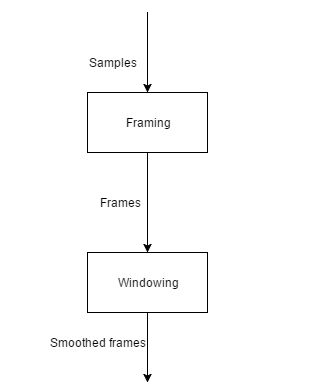
\includegraphics[width=130mm]{resources/mehang/methodology/audiosignalpreprocessing}
        \caption{Block Diagram of Audio Signal Pre-processing}
\end{figure}

\subsubsection{Framing}
Framing is the process of dividing the whole audio sample into frames. An audio signal is constantly changing, so we assume that on short time scales the audio signal doesn’t change ( when we say it doesn’t change, we mean statistically stationary, obviously the samples are constantly changing on even short time scales). This is why we frame the signal into 20-40 ms frames. If the frame is much shorter we don’t have enough samples to get a reliable spectral estimate, if it is longer the signal changes too much throughout the frame.So, a frame provides a redundant, stable way of representing a signal.
To mitigate the “loss” at the edges of the window, the frames may overlap in time.

\subsubsection{Windowing}
Windowing refers to the processing of multiplying of frames with the window function like rectangular window, hamming window, hanning window etc. Windowing are necessary because whenever we do a finite Fourier transform, it is implicitly being applied to an infinite repeating signal. So, for instance if the start and end of a finite sample doesn’t match then that will look just like a discontinuity in the signal, and show up a lots of high-frequency noise in the Fourier Transform, which is harmful. If the sample happens to be a perfect sinusoid but with an integer number of periods then it doesn’t fit exactly into the finite sample and the FT will show appreciable energy in all sorts of places nowhere near the real frequency. So windowing make sure that the end matchup while keeping everything reasonably smooth.
\begin{figure}[h!]
        \centering
        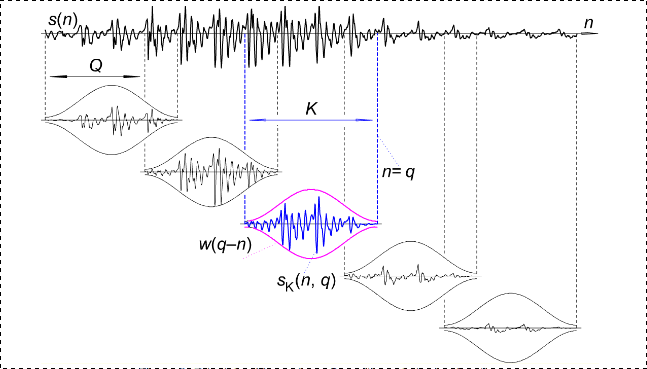
\includegraphics[width=130mm]{resources/mehang/methodology/framingandwindowing}
        \caption{Principle of frame formation and windowing function}
\end{figure}
where s(n) denotes the sampled speech signal,\\
Q is the frame length,\\
K is the window length,\\
q is the sample point the window is applied,\\
and $s_k$(n,q) is a resulting short time signal, with $s_k$(n,q) = s(n)w(q-n).

\subsection{Feature Extraction}
Feature extraction starts from an initial set of measured data and builds derived values (features) intended to be informative and non-redundant, facilitating the subsequent learning and generalization steps, and in some cases leading to better human interpretations. Feature extraction is related to dimensionality reduction.\\
\\
The feature extraction procedure is depicted in the following figure.
\begin{figure}[h!]
        \centering
        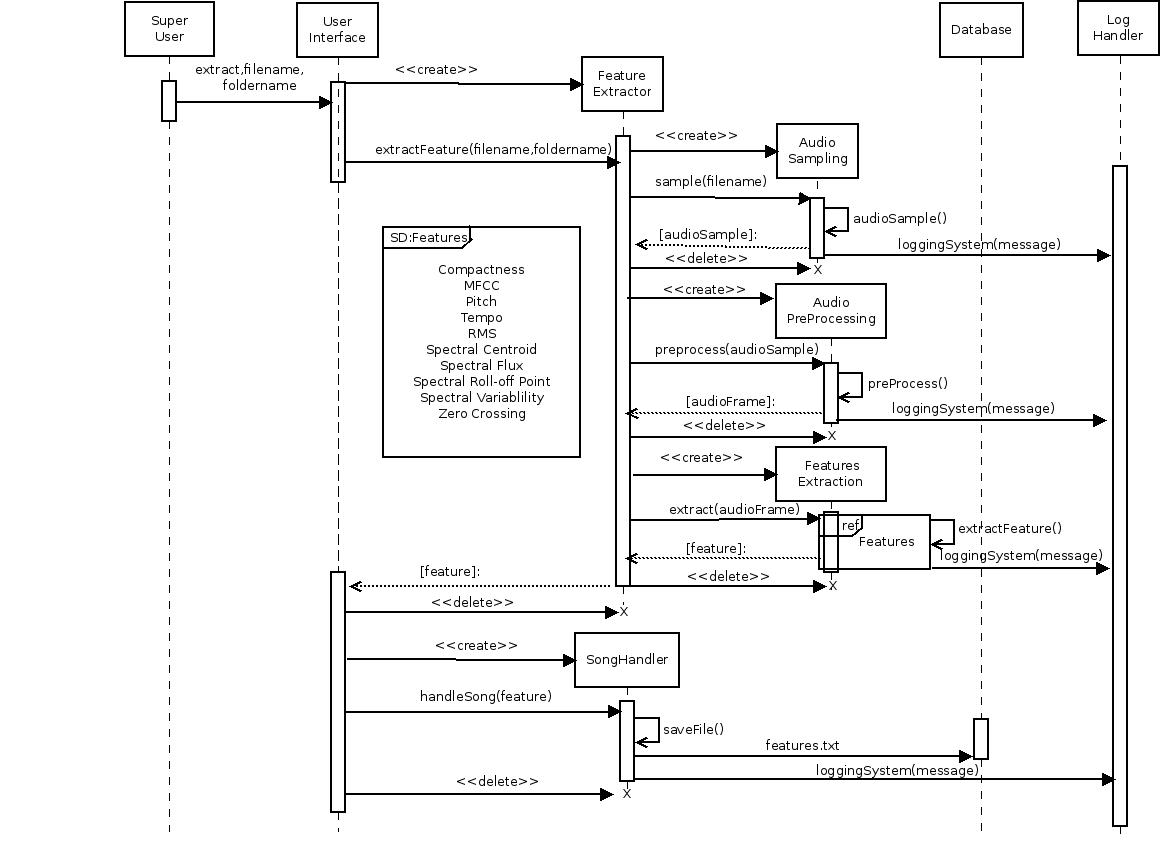
\includegraphics[width=130mm]{resources/mehang/methodology/featureextraction}
        \caption{Block Diagram of Feature extraction}
\end{figure}

\subsubsection{Fast Fourier Transform}
A Fast Fourier Transform(FFT) algorithm computes the DFT(Discrete Fourier Transform) of a sequence, or its inverse. Fourier analysis converts a signal from its original domain (often time or space) to a representation in the frequency domain and vice versa. An FFT rapidly computes such transformation by factorizing the DFT matrix into a product of sparse (mostly zero) factors. As a result, it manages to reduce the complexity of computing the DFT from O($n^2$) which arises if one simply applies the definition of the DFT to O(nlogn), where n is the data size. 

\subsubsection{Magnitude Spectrum}
Magnitude Spectrum is the magnitude of different frequency components within a window. The magnitude spectrum is found by first calculating the FFT within window. The magnitude spectrum value for each bin is found by first summing the squares of the real and imaginary components. The square root of this is then found and the result is divided by the number of bins.

\subsubsection{Power Spectrum}
Power Spectrum is the power of different frequency components within a window. The power spectrum is found by first calculating the FFT with a Hanning window. The magnitude spectrum value for each bin is found by first summing the squares of the real and imaginary components. The result is divided by the number of bins.

\subsubsection{Compactness}
It is the measure of the noisiness of a signal. It is found by comparing the 
components of a window’s magnitude spectrum with the magnitude spectrum of its  
neighbouring windows.\\ 
\\
If M[n], M[n-1] and M[n+1] $>$ 0, then
\begin{equation}
        compactness = \sum_{n=2}^{N-1}{((|20*log(M[n]))-20*(log(M[n-1])+log(M[n])+log(M[n+1]))]/3|)}
\end{equation}
otherwise,
\begin{equation}
        compactness = 0
\end{equation}
where M[n] is the Magnitude Spectrum at internal n.

\subsubsection{Mel-Frequency Cepstral Coefficients}
It is a representation of the short-term power spectrum of a sound, based on a linear cosine 
transform of a log power spectrum on a nonlinear mel scale of frequency.\\
\\
\textbf{Algorithm}
\begin{enumerate}[(i)]
        \item \textbf{Framing:}
                The process of segmenting the speech samples obtained from analog to digital conversion(ADC) into a small frame with the length within
                the range of 20 to 40 msec. The voice signal is divided into frames of Nsamples. Adjacent frames are being separated by M(M $<$ N).
        \item \textbf{Hamming Window:}
                Hamming window is used as window shape by considering the next block in feature extraction processing chain and integrates all the 
                closest frequency lines. The Hamming window equation is given as:\\
                \\
                If the window is defines as W(n), 0 $\le$ n $\le$ N-1 where\\
                N = number of samples in each frame\\
                Y[n] = Output signal
                X(n) = Input signal
                W(n) = Hamming window,\\
                then the result of windowing signal is shown below:
                \begin{equation}
                        Y(n) = X(n) \times W(n)
                \end{equation}
                \begin{equation}
                        W(n) = 0.54 - 0.46cos\Big(\frac{2 \pi n}{N-1}\Big), \hspace{10mm}0 \le n \le N-1
                \end{equation}
        \item \textbf{Fast Fourier Transform:}
                To convert each frame of N samples from time domain into frequency domain. The Fourier Transform is to convert the
                convolution of the glottal pulse U[n] and the vocal tract impulse response H[n] in the time domain. This statement supports the equation below:
                \begin{equation}
                        Y(w) = FFT[h(t)*X(t)] = H(w) * X(w)
                \end{equation}
                If X(w), H(w) and Y(w) are the Fourier Transform of X(t), H(t) and Y(t) respectively.
        \item \textbf{Mel Filter Bank Processing:}
                The frequencies range in FFT spectrum is very wide
                and voice signal does not follow the linear scale as shown in figure 4.5 is then
                performed. This figure shows a set of triangular filters that are used to
                compute a weights sum of filter spectral components so that the output of
                process approximates to a Mel scale. Each filter’s magnitude frequency re-
                sponse is triangular in shape and equal to unity at the centre frequency and
                decrease linearly to zero at centre frequency of two adjacent filters [7,8].
                Then, each filter output is the sum of its filtered spectral components. After
                that the following equation is used to compute the Mel for given frequency
                f in Hz:
                \begin{figure}[h!]
                        \centering
                        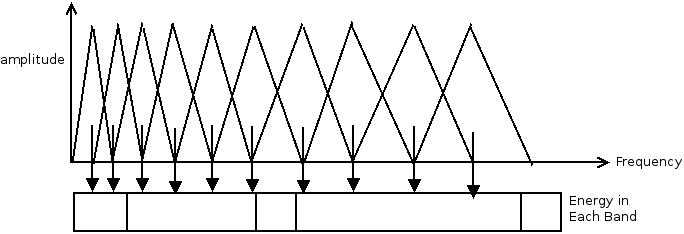
\includegraphics[width=150mm]{resources/melscale}
                        \caption{Mel scale filter bank}
                        \label{fig:Melscale}
                \end{figure}
                This figure shows a set of triangular filters that are used to compute a weights sum of filter spectral components so that the output
                of process approximates to a Mel scale. Each filter's magnitude frequency response is triangular in shape and equal to unity at the
                centre frequency and decrease linearly to zero at centre frequency of two adjacent filters [7,8]. Then, each filter output is the sum of its
                filtered spectral components. After that the following equation is used to compute the Mel for given frequency f in Hz:
                \begin{equation}
                        M(f) = 1125ln\Big(1+\frac{f}{700}\Big)
                \end{equation}
        \item \textbf{Discrete Cosine Transform:}
                This is the process to convert the log Mel spectrum into time domain using Discrete Cosine Transform(DCT). The result of the conversion is
                called Mel Frequency Cepstrum Coefficient. The set of coefficient is called acoustic vectors. Therefore, each input utterance is transformed
                into a sequence of acoustic vector.
\end{enumerate}

\subsubsection{Pitch}
It is a perceptual property of sounds that allows their ordering on a frequency­related scale, or 
more commonly, pitch is the quality that makes it possible to judge sounds as "higher" and "lower" in 
the sense associated with musical melodies.\\  
\\
It is a subjective psychoacoustical attribute of sound, and hence is approximately quantified 
as fundamental frequency.Pitch is an auditory sensation in which a listener assigns musical tones to 
relative positions on a musical scale based primarily on their perception of the frequency of 
vibration.Pitch is closely related to frequency, but the two are not equivalent. Frequency is an 
objective, scientific attribute that can be measured. Pitch is each person's subjective perception  of a 
sound wave, which cannot be directly measured. However, this does not necessarily mean that most 
people won't agree on which notes are higher and lower.\\ 
\\
\textbf{Algorithm}
\begin{enumerate}[(i)]
        \item Model the signal $x_t$ as a periodic function with period T, by definition invariant for a time shift
                of T
                \begin{equation}
                        x_t - x_{t+T} = 0,\hspace{10mm}\forall t
                \end{equation}
                The same is true after taking the square and averaging over a window
                \begin{equation}
                        \sum_{d=t+1}^{t+W}{(x(j)-x(j+\tau))^2} = 0
                \end{equation}
                    Conversely, an unknown period may be found by forming a difference function and searching for 
                    the values of $\tau$ for which the function is zero.
            \item The cumulative mean normalized difference function is calculated by dividing each value of the old 
                    by its average over shorter-lag values. It differs from difference function in the first step in that it 
                    starts at one rather than zero, tends to remain large at low lags, and drops below one only where the first 
                    difference function falls below average. 
            \item Set an absolute threshold and choose the smallest value of $\tau$ that gives a minimum of the  
                    difference function obtained in the second step deeper than that threshold. If none is found, the 
                    global minimum is chosen instead. With a threshold of 0.1, the error rate drops significantly. 
            \item Each local minimum of the second difference function and its immediate neighbors is fit by a 
                    parabola, and the ordinate of the interpolated minimum is used in the dip-selection process. The 
                    abscissa of the selected minimum then serves as a period estimate. Actually, one finds that the 
                    estimate obtained in this way is slightly biased. To avoid this bias, the abscissa of the corresponding 
                    minimum of the raw difference function(the first) is used instead. 
\end{enumerate}

\subsubsection{Tempo}
The beat is the regularly occurring pattern of rhythmic stresses in music. When we count, tap or clap along 
with music we are experiencing the beat. Try tapping your finger along with different types of music and see 
what happens.\\ 
\\
Tempo is the speed of the beat, usually expressed in Beats Per Minute(BPM). For example, at 120 BPM 
there will be 120 beats in one minute. Tempo can also be expressed verbally with different music terms, 
such as Slowly, Fast, Allegro, or Largo.\\
\\
\textbf{Algorithm}
\begin{enumerate}[(i)]
        \item Parse an audio file into samples, s[n], with a corresponding sampling rate, SR.
        \item Break the audio file into N windows of 1024 samples.
        \item Calculate the FFT of each window.
        \item Calculate the power spectrum(P) of each window form the corresponding FFT results.
        \item Calculate the spectral flux(F) from the power spectrum(P) of each window, i:
                \begin{equation}
                        F_i = (P_i - P_{i-1})^2
                \end{equation}
        \item Find the mean flux, $F_{av}$, across all windows.
        \item Set $F_i$, the flux for each window, to 0 if it is not at least 1.5 times $F_{av}$ (this value
                was experimentally determined). This gives a generous estimation of note onsets.
        \item Use autocorrelation to find the histogram of lag frequencies, L:
                \begin{equation}
                        L[lag] = \sum_{i}^{N}{F[i]F[i+lag]}
                \end{equation}
        \item Calculate the effective sampling rate, $S_{eff}$, found in F and L.
                \begin{equation}
                        SR_{eff} = \frac{SR}{1024}
                \end{equation}
        \item Convert the lag histogram L[lag] into a tempo histogram L[BPM] with bins of beats per
                minute by reversing the order of L and converting the bin lag indices, lag, to BPM:
                \begin{equation}
                        L[BPM] = L\Big(\frac{60*SR_{eff}}{lag}\Big)
                \end{equation}
        \item The result of step (x), L[BPM], is a tempo histogram with bin labels corresponding to beats 
                per minute and bin frequencies correspoding to frequencies of inter-peak intervals.

\end{enumerate}
\subsubsection{Root Mean Square}
The root mean square(abbreviated RMS of rms) is defined as the square root of mean square(the arithmetic mean
of the squares of a set of numbers).
\begin{equation}
        x_{rms} = \sqrt{\frac{1}{n}(x_1^2+x_1^2+...+x_n^2)}
\end{equation}
where there is set of n values \{$x_1, x_2, ......., x_n$\}.

\subsubsection{Spectral Centroid}
The spectral centroid is defined as the center of gravity of the magnitude spectrum of the STFT.
\begin{equation}
        C_t = \frac{\sum\limits_{n=1}^{N}{M_t[n]*n}}{\sum\limits_{n=1}^{N}{M_t[n]}}
\end{equation}
where $M_t[n]$ is the magnitude of the Fourier transform at frame t and frequency bin n.\\
The centroid is a measure of spectral shape and higher centroid values correspond to "brighter" textures with more high frequencies.

\subsubsection{Spectral Flux}
The spectral flux is defined as the squared difference between the normalized magnitudes of successive spectral distributions.
\begin{equation}
        F_t = \sum_{n=1}^{N}{(N_t[n]-N_{t-1}[n])^2}
\end{equation}
where $N_t[n]$ and $N_{t-1}[n]$ are the normalized magnitude of the Fourier transform at the current frame t, and the previous frame t-1, 
respectively.\\ 
The spectral flux is a measure of the amount of local spectral change.

\subsubsection{Spectral Roll-off Point}
The spectral roll-off is defined as the frequency $R_t$ below which 85 per cent of the magnitude distribution is concentrated.
\begin{equation}
        \sum_{n=1}^{R_t}M_t[n] = 0.85*\sum_{n=1}^{N}{M_t[n]}
\end{equation}
The roll-off is another measure of spectral shape.

\subsubsection{Spectral Variability}
  Spectral variability is the standard deviation of the magnitude spectrum. This gives the 
  measure of the variance of a signal's magnitude spectrum. 
  \begin{equation}
          Spectral variability = \sqrt{\frac{1}{N-1}-(\sum_{n=1}^{N}{M[n]-mean})^2}
  \end{equation}
  where M[n] = Magnitude spectrum of the signal at interval n,
  Mean = mean of the magnitude spectrum.

\subsubsection{Zero Crossing}
The zero crossing is defined as the number of times the waveform changed sign.
\begin{equation}
        Z_t = \frac{1}{2}\sum_{n=1}^{N}{|sign(x[n])-sign(x[n-1])|}
\end{equation}
where the sign fucntion is 1 for positive arguments and 0 for negative arguments and\\
x[n] is the time domain signal for frame t.\\
Time domain zero crossings provide a measure of the noisiness of the signal.
\newpage
\subsection{Feature Integration}
Feature Integration is the processing of integrating the various significant features obtained by the feature extraction process.\\
\\
The feature integration procedure is depicted in the following figure.
\begin{figure}[h!]
        \centering
        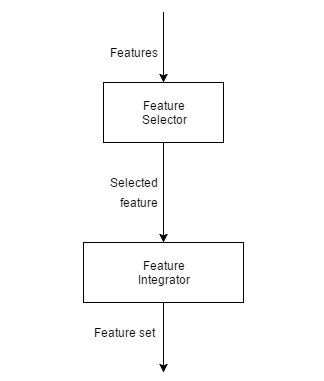
\includegraphics[width=130mm]{resources/mehang/methodology/featureintegration}
        \caption{Block Diagram of Feature integration}
\end{figure}

\subsubsection{Feature Selector}
Feature selector perform the feature selection process. Feature selection, also known as variable 
selection, attribute selection or variable subset selection, is the process of selecting a subset of relevant features( variable, predictors) for use in model construction. Feature selection technique are used for the three reasons:
\begin{enumerate}[(i)]
        \item Simplification of models to make them easier to interpret by researchers/users
        \item Shorter training time
        \item Enhanced generalization by reducing overfitting
\end{enumerate}

\subsubsection{Feature Integrator}
Feature integrator merges the features selected by Feature Selector into one set for each song.
As the features are temporal, so the feature integration is also temporal.
Feature integration is the process of combining all the feature vectors in a time window into a single feature vector in order to capture the relevant temporal information in the window. 
In this project, the mean and variance of the features have been used for temporal feature integration
although they capture neither the temporal dynamics nor dependencies among the individual feature dimensions.

As seen below, the mean and standard deviation of MFCCs for a classical and a hiphop songs are sufficiently distinguishable. 
So, this representation of the features can be used to separate classes of music.
\begin{figure}[h!]
        \centering
        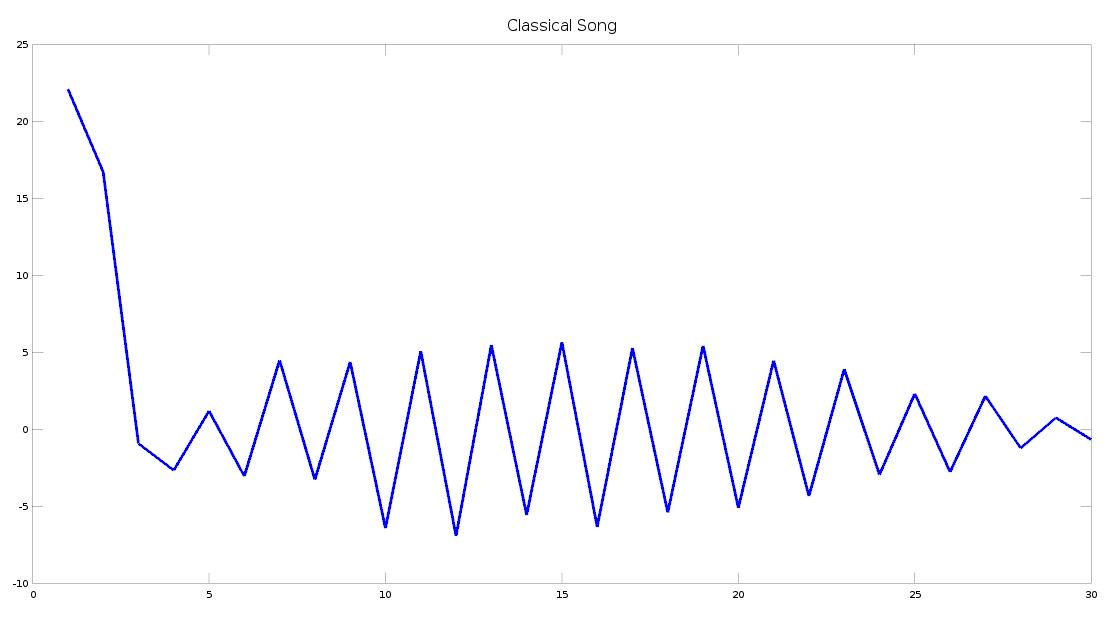
\includegraphics[width=70mm]{resources/mehang/4.5.2/MFCC_mean_Classical}
        \caption{Mean of MFCC for a  classical song}
\end{figure}
\begin{figure}[h!]
        \centering
        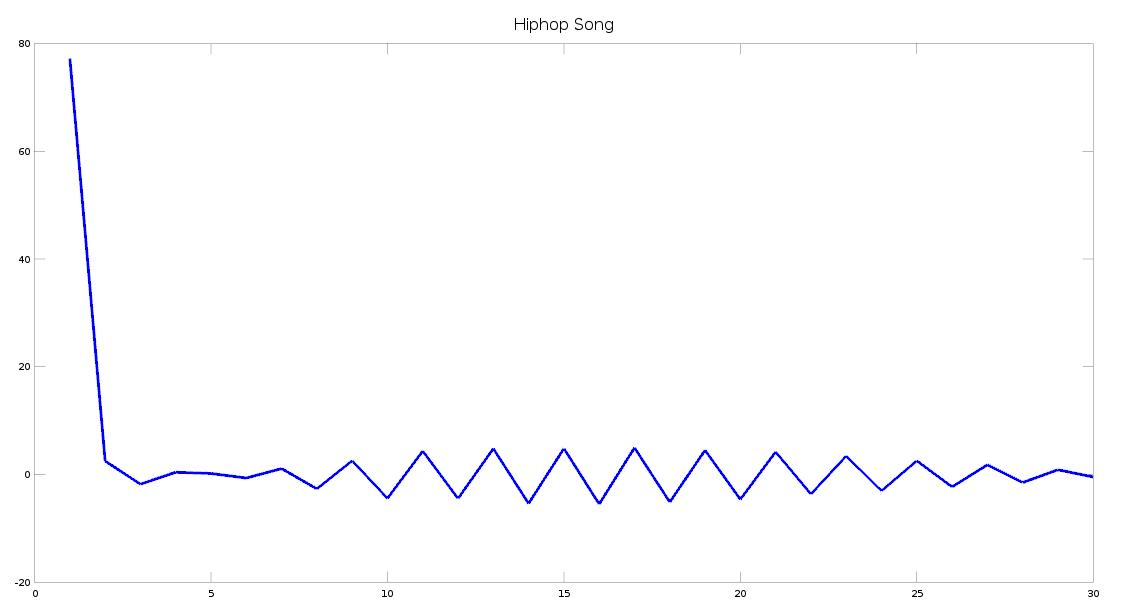
\includegraphics[width=70mm]{resources/mehang/4.5.2/MFCC_mean_Hiphop}
        \caption{Mean of MFCC for a hiphop song}
\end{figure}
\begin{figure}[h!]
        \centering
        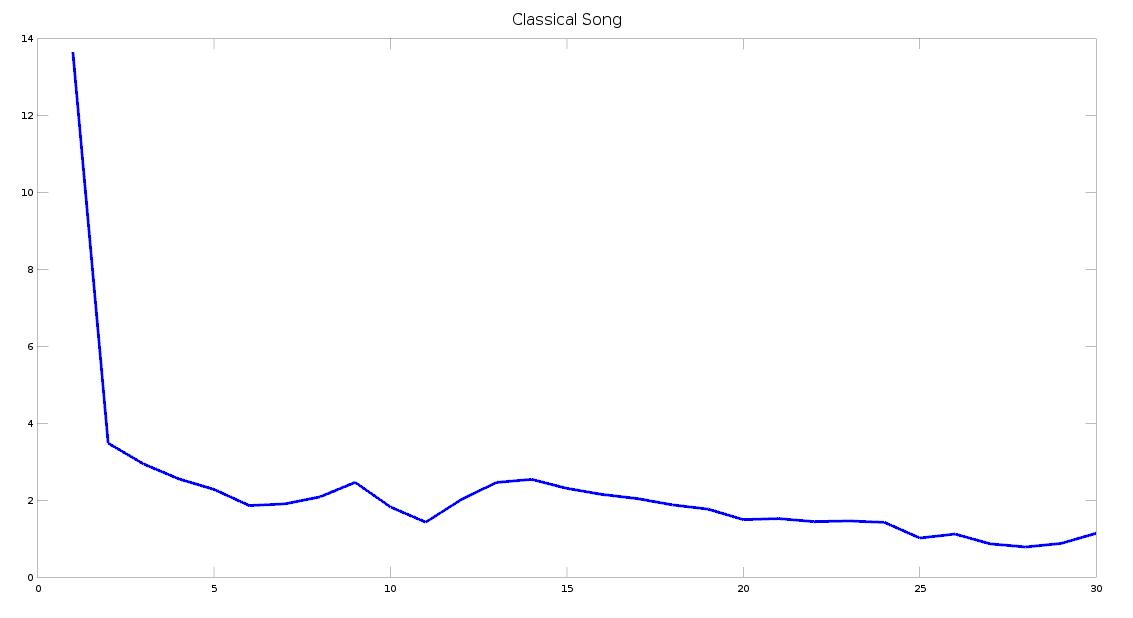
\includegraphics[width=70mm]{resources/mehang/4.5.2/MFCC_sd_Classical}
        \caption{Standard deviation of MFCC for a classical song}
\end{figure}
\begin{figure}[h!]
        \centering
        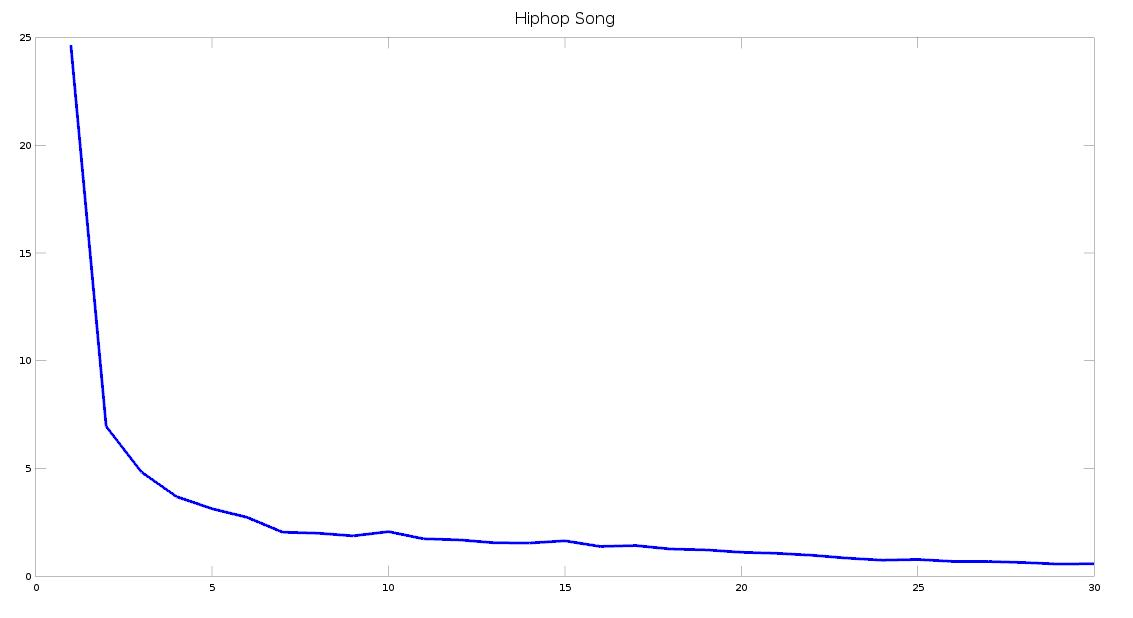
\includegraphics[width=70mm]{resources/mehang/4.5.2/MFCC_sd_Hiphop}
        \caption{Standard deviation of MFCC for a hiphop song}
\end{figure}


\newpage


\subsection{Classification}
\begin{figure}[h!]
        \centering
        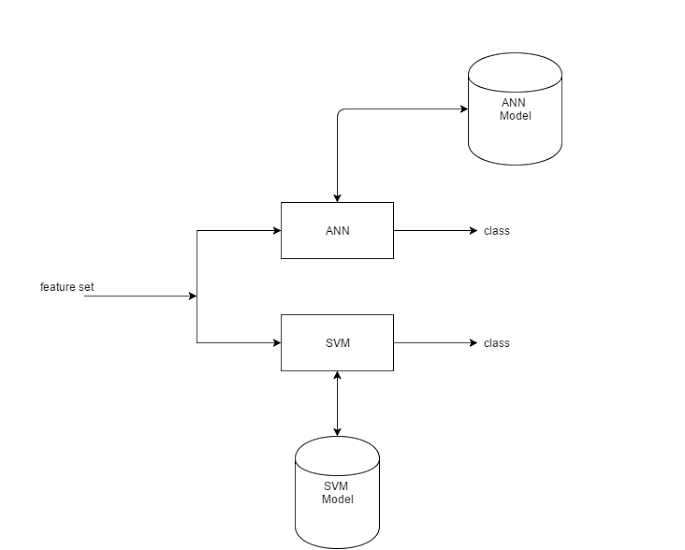
\includegraphics[width=130mm]{resources/mehang/methodology/classification}
        \caption{Block Diagram of the Classification Step}
\end{figure}

\subsubsection{Artificial Neural Network.}
In machine learning and cognitive science, an artificial neural networks(ANN) is a network inspired by biological neural networks(the central nervous systems of 
animals, in particular the brain) which are used to estimate or approxiamte functions that can depend on a large numbers of inputs that are generally unknown.
Our research shows whether the research is related to our field or other, most of the time for machine learning researchers used artificial neural network.
So our choice was simple as it was based on supervised learning and comparatively simple than other complicated unsupervised learning.
Research papers \cite{Kour2015},\cite{Anglade2010}, \cite{Neumayer2004}  ,\cite{Koerich2013},\cite{Koerich2013}and \cite{Haggblade2011}   shows the implementation of artificial neural network in the field of
music classification.\\
\\
Artificial neural networks are typically specified using three things:
\begin{itemize}
        \item \textbf{Architecture:} 
                It specifies what variables are involved in the network and their topological relationships- for example the variable involved
                in a neural network might be the weights of the connections between the neurons, along with activities of the neurons. In an artificial
                neural network, there are one or more hidden layers in between input and output layers with all the neurons connecting to each other.
        \item \textbf{Activity Rule:}
                Most neural network models have short tiem-scale dynamic: local rules define how the activities of the neurons change in reponse to each other.
                Typically the activity rule depends on the weights(the parameters) in the network.Here in our case, the set of input neuronse
                is activated by the feature values like MFCC, pitch,etc. There activation function present to trigger the respective neuron. Most of the time
                activation function are non linear, differential mathematical functions like sigmoid, hyperbolic tangent, etc.
        \item \textbf{Learning Rule:}
                The learning rule specifies the way in which the neural network's weights change with time as the learning takes progress. This learning is usually viewed as 
                taking place on a longer time place than time scale of the dynamicx under the activity rule. Usually the learning rule will depend on the activites of the 
                neurons. In our case the learning depends on the values of the target values supplied by a teacher and on the current value of the weights.
\end{itemize}

\begin{figure}[h!]
        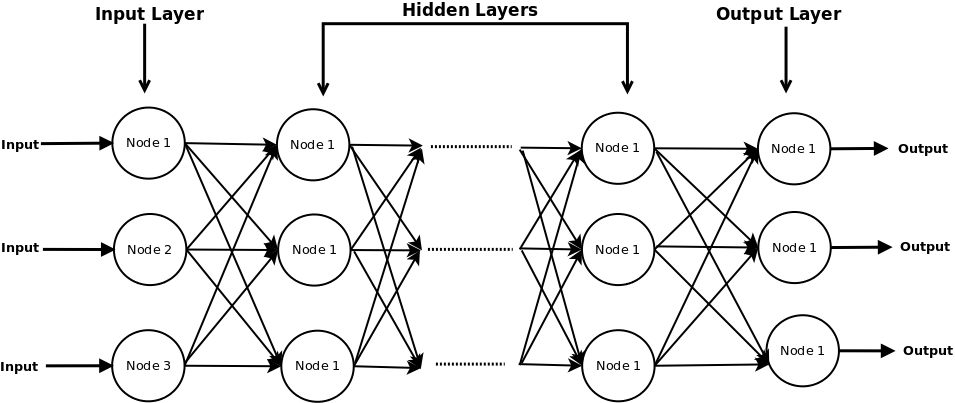
\includegraphics[width=150mm]{resources/ann}
        \caption{General structure of artificial neural network}
\end{figure}
For a system, generally the architecture is created as per the need. Generally for that there is lot of trial and error methodology involved
to determine the correct number of hidden layers and neurons needed. In most cases, one hidden layer is suffiecient for the system but if 
the nature of system or data is perplexing then in accordance to expected result and current behavior, number of hidden layers of nodes can be increased.\\
\\
The concept of cost function is an important in context of artificial neural network. It measures how far away a particular solution is from an
optimal solution. We can also say that the cost of the optimal solution is minimum. So, the target of our artifical neural network is to
try to meet the cost of optimal solution. While it is possible to define some arbitrary ad hoc cost fucntion, frequently a particular cost will be used, either
because it has desirable properties (such as convexity) or because it arises naturally from a particular formulation of problem. Ultimately, the cost
fucntion will depend on the desired task. One of the mostly used cost function is squared error measure between the output value O and the target value t.
\begin{equation}
        E = (t-y)^2
\end{equation}
where E is the discrepancy or error.\\
\\
Using this cost, the neural network tries to adjust its weights in order to minimize the cost function. This is the learning process.
Supervised learning, unsupervised learning and reinforcement learning are the three major paradigms of learning. We are opting for supervised learning as
unsupervised learning and reinforcement learning are comparatively more complex and also supervised learning has been doing a
great job in the field of music classification \cite{Neumayer2004}, \cite{Haggblade2011}, \cite{Kour2015}. Supervised learning 
requires the correct class label to be provided along with the training dataset for the neural network so that it can adjust it's weight based on the cost function 
of incorrect/correct class prediction. Backpropagation algorithm is the most popular learning algorithm for neural network out there. The reason for
its popularity might be its simplicity in terms of concept and wide applicability. It's also based on supervised learning. When one tries to minimize cost function
using gradient descent for the class of neural networks called multilayer perceptrons(MLP), one obtains the common and well-known backpropagation algorithm for training neural networks.\\
\\
Backpropagation is a common method of training artificial neural networks used in conjunction with an optimization method such as gradient descent. The 
method calculates the gradient of a loss function with respect to all the weights in the network. The gradient is fed to the optimization method wihich in turn uses it to
update the weights, in an attempt to minimize the loss function. It is a generalization of delta rule to multi-layered feedforward networks, made possible
by using the chain rule to iteratively compute gradients for each layer. Requirements of backpropagation mehod are:
\begin{itemize}
        \item It requires a known, desired output for each input value in order to calculate the loss function gradient.
        \item It requires the activation function used by the artificial neurons/nodes to be differentiable.
\end{itemize}
\textbf{Algorithm}
\begin{enumerate}[(i)]
        \item Run the network forward with your input data to get the network output.
        \item For each output node compute
                \begin{equation}
                        \delta_k = O_k(1 - O_k)(O_k - t_k)
                \end{equation}
        \item For each hidden node calculate
                \begin{equation}
                        \delta_j = O_k(1 - O_k) \sum_{k \in K}{\delta_kW_{jk}}
                \end{equation}
        \item Update the weights and biases as follows:\\
                Given
                \begin{equation}
                        W = -\eta \delta_l O_{l-1}
                \end{equation}
                \begin{equation}
                        \Delta \theta = -\eta \delta_l
                \end{equation}
                apply
                \begin{equation}
                        W + \Delta W \to W
                \end{equation}
                \begin{equation}
                        \theta + \Delta\theta \to \theta
                \end{equation}
\end{enumerate}
where i, j and k represents the input layer, hidden layer and ouput layer respectively,\\
O is the output of a neuron/node,\\
t is the target value,\\
K is the total number of output neurons/nodes,\\
$\Delta$ represent the difference,\\
l denotes every layer.\\
\\
$\eta$ is the learning rate which is defined as the ratio(percentage) that influences the speed and quality of learning.The greater the ratio, the faster the neuron trains;
the lower the ratio, the more accurate the training is. $\theta$ is the bias term which is involved in adjusting the shifting of activation function. The sign of the gradient
of a weight indicates where the error is increasing, this is why the weight must be updated in the opposite direction. The algorithm above is
repeated until performance of the network is satisfactory.

\subsubsection{ANN model}
It stores the relevant parameters obtained from ANN training for future use without having to retrain.

\subsubsection{Support Vector Machine.}

In machine learning, support vector machines (SVM) are supervised learning models with 
associated learning algorithms that analyze data used for classification analysis.They are new statistical learning technique that can be seen as a new method for training
classifiers based on polynomial functions, radial basis functions, neural networks, splines or other functions. The popularity of Support Vector machine is huge as lot of researcher papers
  \cite{Kour2015},\cite{Anglade2010}, \cite{Koerich2013} and \cite{Haggblade2011} shows its implementation. Not only in the field of music classification but also on various artificial intelligence field like handwriting
recognition, biological and other sciences. It was also able to overthrow general neural network until the advent of deep learning.\\
\\
The basic support vector machine (SVM) is a binary linear classifier which chooses the hyperplane that represents the largest separation, or margin, between the two classes. So  Support vector machines use
a hyperplane to create a classifier. If such a hyperplane exists, it is known as the maximum­margin hyperplane and the linear classifier it defines is known as a maximum margin classifier. 
If there exists no hyperplane that can perfectly split the positive and negative instances, the soft 
margin method will choose a hyperplane that splits the instances as cleanly as possible, while still 
maximizing the distance to the nearest cleanly split instances. For problems that cannot be linearly separated in the input space, this machine offers a possibility to find a solution by making 
a non-linear transformation of the original input space into a high dimension feature space where an optimal separating hyper plane can be found. Those separating planes are optimal, which means
that a maximal margin classifier with respect to the training data set can be obtained. It is developed by Vladimir Vapnik and co-workers at AT\&T Bell Laboratories in 1995.\\
\begin{figure}[h!]
        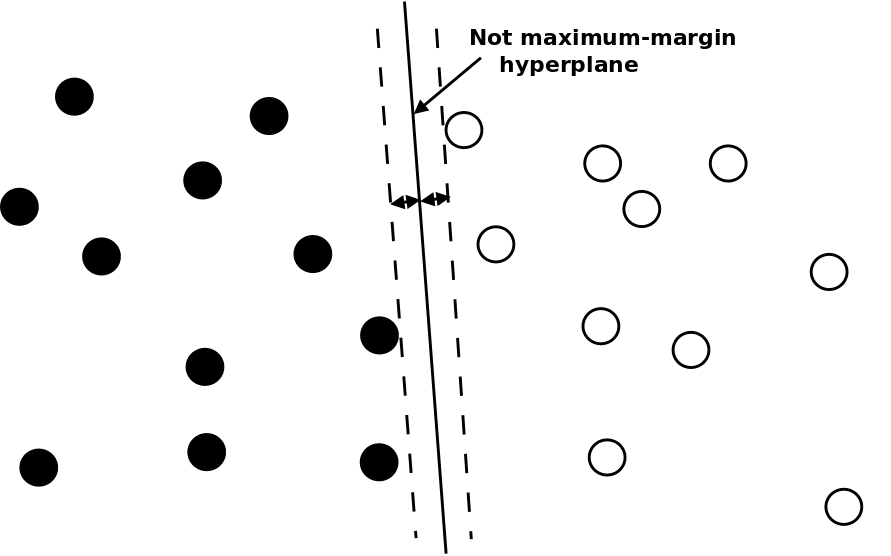
\includegraphics[width=120mm]{resources/misleadinghyperplane}
        \caption{Misleading hyperplane}
\end{figure}
\begin{figure}[h!]
        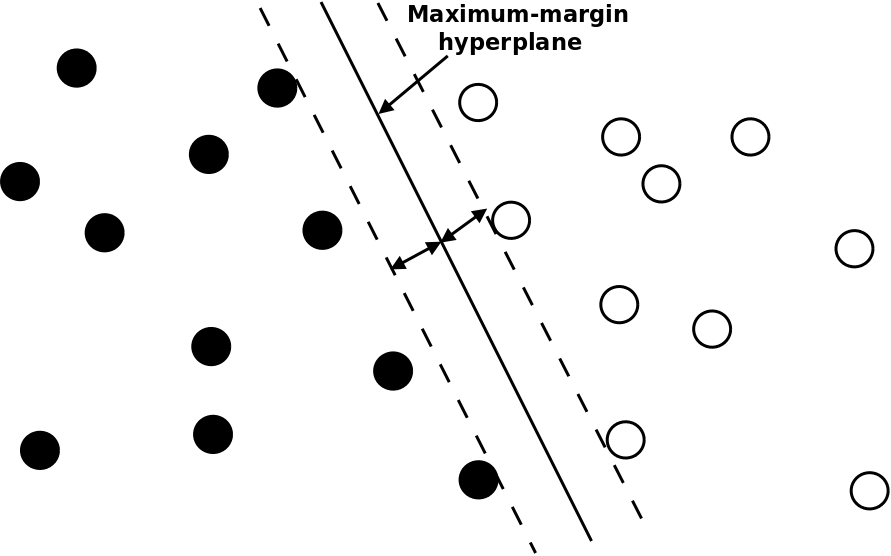
\includegraphics[width=120mm]{resources/svm}
        \caption{Support vector machine with maximum-margin hyperplane}
\end{figure}
The nonlinear SVMs are created by applying the kernel trick to maximum­margin hyperplanes. 
The resulting algorithm is formally similar, except that every dot product is replaced by a nonlinear kernel 
function.\\
\\
\textbf{Kernel Function}\\
The simplest way to divide two groups is with a straight line, flat plane or an N-dimensional hyper plane.
But what if the points are separated by a non-linear region. In such case we would need a non-linear dividing line. Rather than fitting
non-linear curves to the data, support vector machine handles this by using a kernel function to map the data into a different space where
a hyperplane can be used to do the separation. \cite{Anglade2010} shows the use of second order polynomial kernel in the support vector machine.
So, kernel function allows the algorithm to fit the maximum­margin hyperplane in a transformed
feature space. The transformation may be nonlinear and the transformed space be high dimensional. For example, the 
feature space corresponding to Gaussian kernel is a Hilbert space of infinite dimension. Thus though the 
classifier is a hyperplane in the high dimensional feature space, it may be nonlinear in the original input 
space. Maximum margin classifiers are well regularized, so the infinite dimension does not spoil the 
result as the separation will be performed even with very complex boundaries.\\

\begin{figure}[h!]
        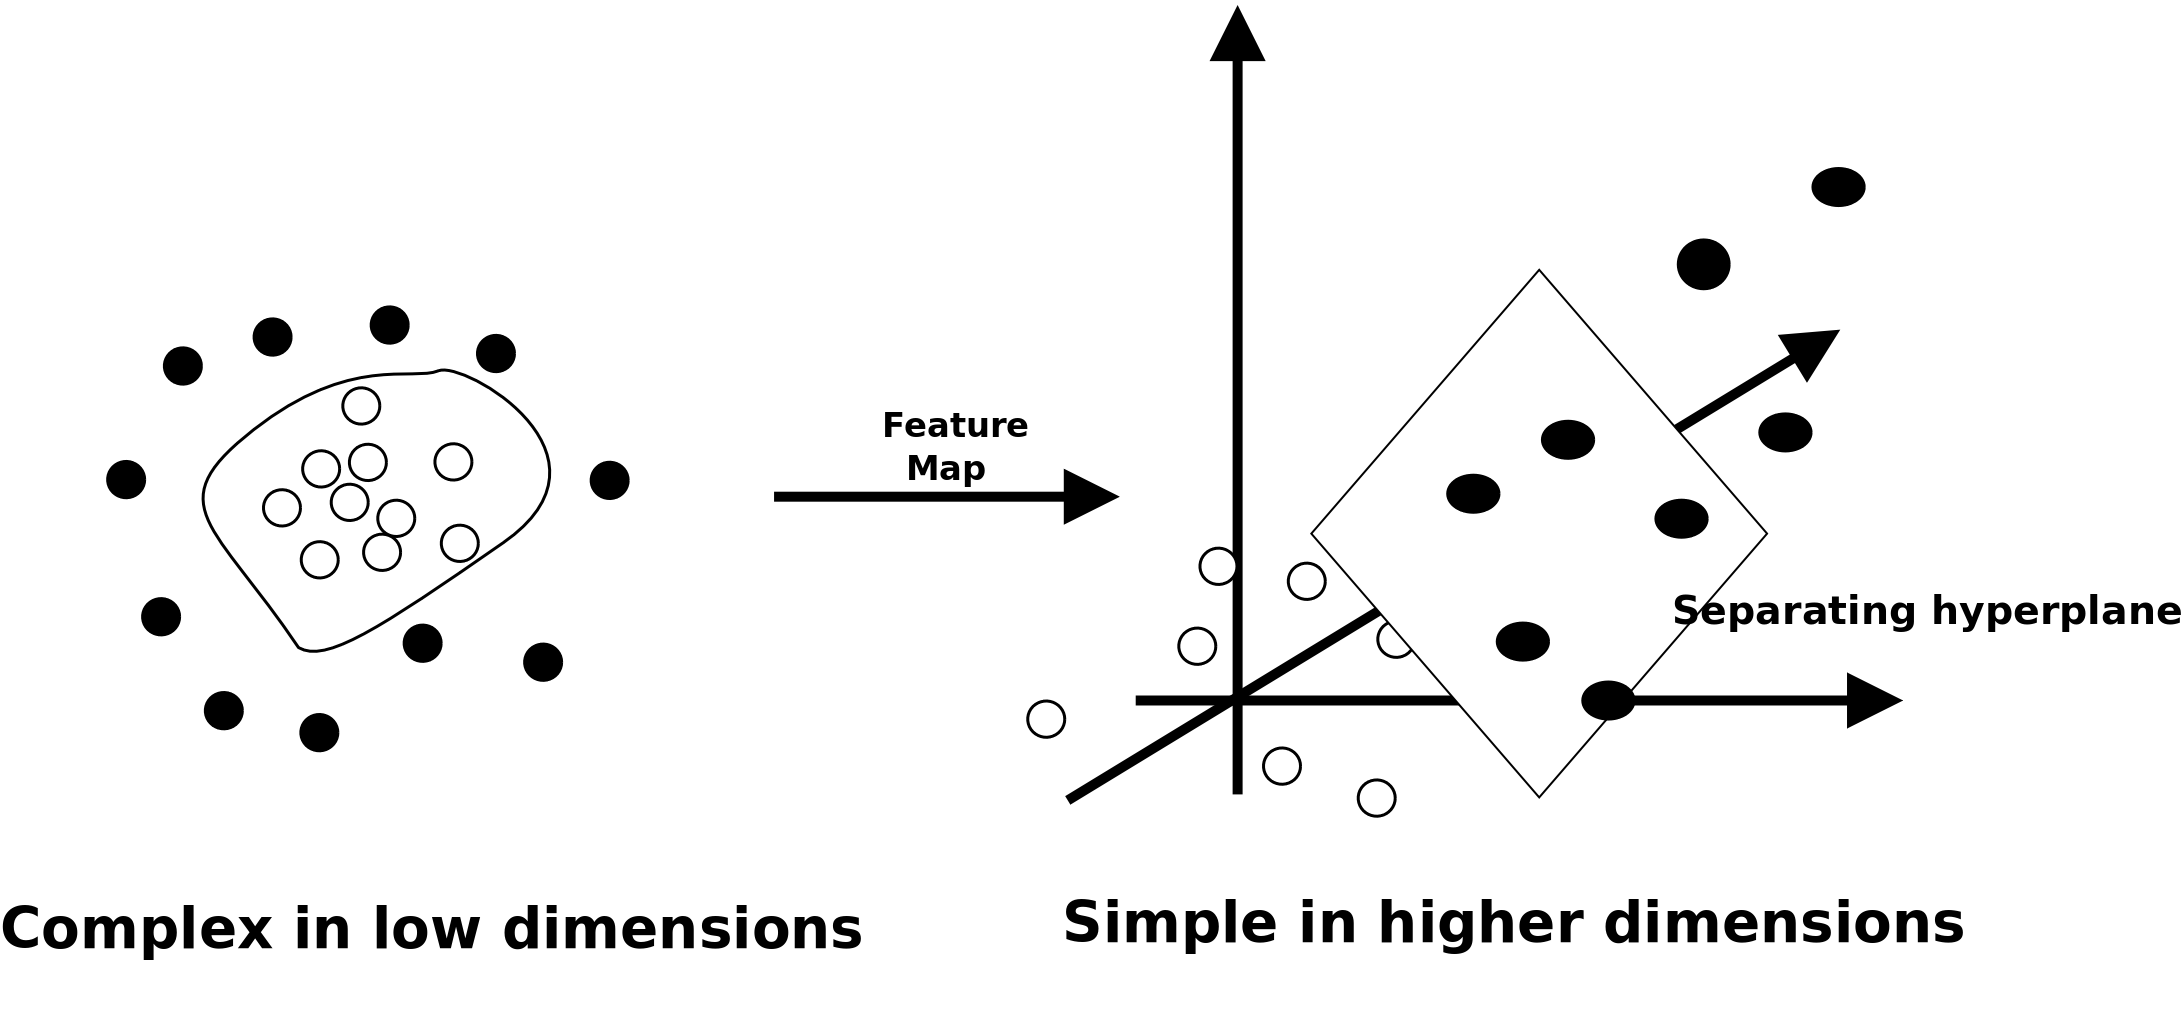
\includegraphics[width=150mm]{resources/kernel}
        \caption{Support vector machine with kernel function}
\end{figure}
\vspace{15mm}
The effectiveness of SVM depends on the selection of kernel, the kernel’s parameters, and soft 
margin parameter c. Given a kernel, best combination of c and kernel’s parameters is often selected by a 
grid­search with cross validation. 
The dominant approach for creating multiclass SVMs is to reduce multi­class problem into 
multiple binary classification problems. Common methods for such reduction is to build binary classifiers 
which distinguish between (i) one of the labels to the rest (one­versus­all) or (ii) between every pair of 
classes (one­versus­one). Classification of new instances for one­versus­all case is done by a 
winner­takes­all strategy, in which the classifier with the highest output function assigns the class. For the 
one ­versus­one approach, classification is done by a max­wins voting strategy, in which every classifier 
assigns the instance to one of the two classes, then the vote for the assigned class is increased by one vote, 
and finally the class with most votes determines the instance classification. To tackle the same multiclass problem \cite{Haggblade2011} has the  
utilization of DAG(Directed Acyclic Graph) SVMs in which a directed acyclic graph(DAG) of two-class SVMs is trained on each pair of classes in the data set.

\subsubsection{SVM model}
It stores the relevant parameters obtained from SVM training for future use without having to retrain.

